\documentclass[11pt,a4paper]{article}

\usepackage{etex} %évite les erreurs no room for ....

\usepackage[french]{babel}
\usepackage[utf8]{inputenc}
\usepackage[T1]{fontenc}
\usepackage{hyperref}
\usepackage{amsmath}
\usepackage{amssymb} %gestion des symboles mathmatiques
\usepackage{amsfonts} %gestion des polices mathmatiques
\usepackage{fancybox} %gestion des encadrements
\usepackage{lastpage} %gestion du nombre total de pages du document
\usepackage{geometry} %gestion des marges du document
\usepackage{fancyhdr} %gestion des entetes et des pieds de page
\usepackage{epsfig}
\usepackage[dvipsnames]{xcolor}
\usepackage{pdftricks}
\usepackage{eurosym}
\usepackage{pifont}
\usepackage{eucal}
\usepackage{multirow}
\usepackage{tabularx}
\usepackage{ulem}
\usepackage{dcolumn}
\usepackage{textcomp}
\usepackage{diagbox}
\usepackage{lscape}
\usepackage{ifpdf}
\usepackage[tikz]{bclogo}
\usepackage{amsthm}
\usepackage{tabvar}
\usepackage{multicol}
\usepackage{frcursive}
\usepackage{color}
\usepackage{colortbl}
\usepackage{pgf,tikz}
\usetikzlibrary{arrows}
\usepackage{eurosym}
\usepackage{cancel}
\usepackage{longtable,booktabs}
\usepackage{tcolorbox}
\tcbuselibrary{skins}
\tcbuselibrary{breakable}
\usepackage{varwidth}
\usepackage{MnSymbol} % contient le caractère \nsubset
\usepackage{wrapfig}
\usepackage{wasysym} % pour certains symboles
\usepackage{minted}
\usepackage{titlesec}
\usepackage[np]{numprint}
\usepackage{fontawesome5}
\usepackage{xspace}
\usepackage{listingsutf8}

\titleformat{\section}
{\Large\bfseries}{\thesection}{1em}{}[\titlerule]
% {\Large\bfseries}{\thesection}{1em}{\MakeUppercase}[\titlerule]

\titleformat{\subsection}
{\large\bfseries}{\thesubsection}{1em}{}[\titlerule]
% {\large\bfseries}{\thesubsection}{1em}{\MakeUppercase}[\titlerule]

%% Macro pour limite  gauche%%
\newcommand{\limgauche}[2]{\lim_{#1\rightarrow #2\hspace{-1.5em}\raisebox{-1.2ex}{\scriptsize $#1<#2$}}}

%% Macro pour limite  droite%%
\newcommand{\limdroite}[2]{\lim_{#1\rightarrow #2\hspace{-1.5em}\raisebox{-1.2ex}{\scriptsize $#1>#2$}}}

\newcommand{\R}{\mathbb{R}}
\newcommand{\N}{\mathbb{N}}
%\newcommand{\D}{\mathbb{D}}
\newcommand{\Z}{\mathbb{Z}}
\newcommand{\Q}{\mathbb{Q}}
\newcommand{\C}{\mathbb{C}}
\newcommand{\lm}[2]{\displaystyle{\lim_{#1 \rightarrow #2}}}
\newcommand{\e}[1]{\text{e}^{#1}}
\renewcommand{\theenumi}{\textbf{\arabic{enumi}}}
\renewcommand{\labelenumi}{\textbf{\theenumi.}}
\renewcommand{\theenumii}{\textbf{\alph{enumii}}}
\renewcommand{\labelenumii}{\textbf{\theenumii.}}
\newcommand{\vect}[1]{\mathchoice%
{\overrightarrow{\displaystyle\mathstrut#1\,\,}}%
{\overrightarrow{\textstyle\mathstrut#1\,\,}}%
{\overrightarrow{\scriptstyle\mathstrut#1\,\,}}%
{\overrightarrow{\scriptscriptstyle\mathstrut#1\,\,}}}
\def\Oij{$\left(\text{O},~\vect{\imath},~\vect{\jmath}\right)$}
\def\Oijk{$\left(\text{O},~\vect{\imath},~ \vect{\jmath},~ \vect{k}\right)$}
\def\Ouv{$\left(\text{O},~\vect{u},~\vect{v}\right)$}
\newcommand{\V}{\overrightarrow}
\newcommand{\Coor}{\binom}
\newcommand{\Rep}{\left(O;\V{i},\V{j}\right)}
\renewcommand{\emph}{\textit}
\setlength{\emergencystretch}{3em} % prevent overfull lines
\providecommand{\tightlist}{\setlength{\itemsep}{0pt}\setlength{\parskip}{0pt}}

\newcommand{\Syst}[2]{\left\{
  \begin{array}{ccccc}
    #1   
    #2
  \end{array}\right.
}

%configuration de listings
\definecolor{couleuroperations}{rgb}{0.6,0.2,1}
\lstset{
backgroundcolor=\color{lightgray!15},
frame=leftline,
%   framexleftmargin=5mm,
rulesepcolor=\color{lightgray},
inputencoding=utf8,
language=python,
basicstyle=\ttfamily\small, %
identifierstyle=\color{black}, %
keywordstyle=\color{MidnightBlue}, %
stringstyle=\color{purple}, %
commentstyle=\it\color{olive}, %
columns=flexible, %
tabsize=2, %
extendedchars=true, %
showspaces=false, %
showstringspaces=false, %
numbers=none, %
numberstyle=\tiny, %
breaklines=true, %
breakautoindent=true, %
captionpos=b,
literate=%
  *{+}{{{\color{couleuroperations}+}}}1
  {-}{{{\color{couleuroperations}-}}}1
  {/}{{{\color{couleuroperations}/}}}1
  {*}{{{\color{couleuroperations}*}}}1
  {=}{{{\color{couleuroperations}=}}}1
  {<}{{{\color{couleuroperations}<}}}1
  {>}{{{\color{couleuroperations}>}}}1
  {\%}{{{\color{couleuroperations}\%}}}1
  {(}{{{\color{couleuroperations}(}}}1
  {)}{{{\color{couleuroperations})}}}1
  {[}{{{\color{couleuroperations}[}}}1
  {]}{{{\color{couleuroperations}]}}}1
  {.}{{{\color{couleuroperations}.}}}1
  {,}{{{\color{couleuroperations},}}}1
  {1}{{{\color{Cyan}1}}}1
  {2}{{{\color{Cyan}2}}}1
  {3}{{{\color{Cyan}3}}}1
  {4}{{{\color{Cyan}4}}}1
  {5}{{{\color{Cyan}5}}}1
  {6}{{{\color{Cyan}6}}}1
  {7}{{{\color{Cyan}7}}}1
  {8}{{{\color{Cyan}8}}}1
  {9}{{{\color{Cyan}9}}}1
  {0}{{{\color{Cyan}0}}}1,
}

%%%%%%%%%%%%%%%%%% MES ENVIRONNEMENTS %%%%%%%%%%%%%%%%%%%%%%%%%%%%%

\newenvironment{definition}[1]{\begin{tcolorbox}[title= {\color{NavyBlue} \faPencil*}~~\textbf{Définition #1}, colframe=NavyBlue, colback=white, colbacktitle=NavyBlue!10!white, coltitle=black, boxrule=0.1mm, titlerule=0mm]}{\end{tcolorbox}}

\newenvironment{info}[1]{\begin{tcolorbox}[title= {\color{ProcessBlue} \faBook}~~\textbf{#1}, colframe=ProcessBlue, colback=white, colbacktitle=ProcessBlue!15!white, coltitle=black, boxrule=0.1mm, titlerule=0mm]}{\end{tcolorbox}}

\newenvironment{remarque}[1]{\begin{tcolorbox}[title= {\color{SkyBlue} \faInfo}~~\textbf{Remarque #1}, colframe=SkyBlue, colback=white, colbacktitle=SkyBlue!20!white, coltitle=black, boxrule=0.1mm, titlerule=0mm]}{\end{tcolorbox}}

\newenvironment{indication}[1]{\begin{tcolorbox}[title= {\color{Turquoise} \faHotjar}~~\textbf{Indication #1}, colframe=Turquoise, colback=white, colbacktitle=Turquoise!15!white, coltitle=black, boxrule=0.1mm, titlerule=0mm]}{\end{tcolorbox}}

\newenvironment{solution}[1]{\begin{tcolorbox}[title= {\color{ForestGreen} \faCheck}~~\textbf{Solution #1}, colframe=ForestGreen, colback=white, colbacktitle=ForestGreen!15!white, coltitle=black, boxrule=0.1mm, titlerule=0mm]}{\end{tcolorbox}}

\newenvironment{exercice}[1]{\begin{tcolorbox}[title= {\color{YellowGreen} \faQuestion}~~\textbf{Exercice #1}, colframe=YellowGreen, colback=white, colbacktitle=YellowGreen!15!white, coltitle=black, boxrule=0.1mm, titlerule=0mm]}{\end{tcolorbox}}

\newenvironment{attention}[1]{\begin{tcolorbox}[title= {\color{Dandelion} \faExclamationTriangle}~~\textbf{Attention #1}, colframe=Dandelion, colback=white, colbacktitle=Dandelion!15!white, coltitle=black, boxrule=0.1mm, titlerule=0mm]}{\end{tcolorbox}}

\newenvironment{avertissement}[1]{\begin{tcolorbox}[title= {\color{RedOrange} \faSkullCrossbones}~~\textbf{#1}, colframe=RedOrange, colback=white, colbacktitle=RedOrange!15!white, coltitle=black, boxrule=0.1mm, titlerule=0mm]}{\end{tcolorbox}}

\newenvironment{theoreme}[1]{\begin{tcolorbox}[title= {\color{red} \faBolt}~~\textbf{Thèorème #1}, colframe=red, colback=white, colbacktitle=red!10!white, coltitle=black, boxrule=0.1mm, titlerule=0mm]}{\end{tcolorbox}}

\newenvironment{exemple}[1]{\begin{tcolorbox}[title= {\color{Periwinkle} \faFlask}~~\textbf{Exemple #1}, colframe=Periwinkle, colback=white, colbacktitle=Periwinkle!10!white, coltitle=black, boxrule=0.1mm, titlerule=0mm]}{\end{tcolorbox}}

\newenvironment{citations}[1]{\begin{tcolorbox}[title= {\color{Gray} \faQuoteRight}~~\textbf{Citation #1}, colframe=Gray, colback=white, colbacktitle=Gray!10!white, coltitle=black, boxrule=0.1mm, titlerule=0mm]}{\end{tcolorbox}}

\geometry{ tmargin=2cm,bmargin=2cm, hmargin=1.5cm }

\everymath{\displaystyle}

\setlength{\parindent}{0cm}

\pagestyle{fancy}

\begin{document}
    
    
    \lhead{Première NSI} \rhead{2022/2023}
    \chead{} 
    \cfoot{}
    \lfoot{Lycée \'Emile Duclaux}
    \rfoot{Page \thepage/\pageref{LastPage}}
    \renewcommand{\headrulewidth}{0pt}
    \renewcommand{\footrulewidth}{0pt}
    
    \Huge S2 - Ch. 5 : Représentation d'un texte en machine  

    \vspace{.25cm}
    \normalsize Cours  
    
    \vspace{.25cm}
    \hrule
    
    \vspace{.5cm}


Une chaîne de caractères est une suite ordonnée de caractères. Ces
caractères peuvent être :

\begin{itemize}
\tightlist
\item
  des lettres minuscules ou majuscules ;
\item
  des symboles de ponctuation ou autres ;
\item
  des chiffres.
\end{itemize}

En machine, les caractères, comme toute autre \emph{information}, est
codée de façon numérique par un nombre binaire.

Le problème qui se pose est que les lettres de l'alphabet, par exemple,
ne sont pas les mêmes dans toutes les langues et des caractères. Il faut
pouvoir coder des caractères aussi divers que : é, à, ô, \ss{}, \(\Delta\),...

Différents systèmes d'\textbf{encodage} des caractères existent.

\begin{info}{À retenir}
   Une représentation informatique des caractères nécessite
d'associer à chaque caractère une unique séquence d'octets. Cette
conversion s'effectue à l'aide d'une \textbf{table de codage} et d'un
\textbf{encodage}.

\begin{itemize}
\tightlist
\item
  Une table de codage ou jeu de caractères ou charset, associe un entier
  nommé point de code à un caractère.
\item
  Un encodage associe à un point de code une séquence d'octets.
\end{itemize}
\end{info}

Pour une table de codage, il peut exister plusieurs encodages : ce sera
le cas pour la table Unicode, présentée ci-dessous, pour laquelle
plusieurs encodages existent (UTF-8, UTF-16, \ldots).

\hypertarget{le-code-ascii}{%
\subsection*{1. Le code ASCII}\label{le-code-ascii}}

Dans les premiers temps de l'informatique, de nombreux systèmes de
codage, incompatibles entre eux, existaient.

En 1960, l'organisation internationale de normalisation (International
Standard Office : ISO) a créé la norme ASCII (American Standard Code for
Information Interchange) pour écrire des textes en anglais.

La table ASCII fournit la correspondance entre 128 caractères et leur
représentation binaire. Les caractères sont numérotés de 0 à 127. Comme
\(2^7=128\), il suffit de 7 bits par caractère. Cependant, un octet est
le plus souvent utilisé, le bit de poids fort, inutilisé, étant toujours
égal à 0.

Dans le code ASCII, les codes des lettres minuscules et des lettres
majuscules diffèrent d'un bit, le cinquième. Par exemple ``G'' est codé
par \(71_{10}=0100\;0111_2\) et ``g'' est codé par
\(103_{10}=0101\;0111_2\). Cela revient à ajouter \(32=2^5\) pour passer
du code de la majuscule au code de la minuscule.

Les chiffres sont codés par le nombre binaire \(0011\;XXXX_2\) où
\(XXXX_2\) est la valeur du chiffre en binaire. Par exemple 5 est codé
par \(0011\;0101_2\).

Le code ASCII d'un caractère étant composé de 8 bits, il peut aussi être
représenté par un nombre hexadécimal à deux chiffres.

\newpage

  

Voici la table ASCII complète :
\begin{center}
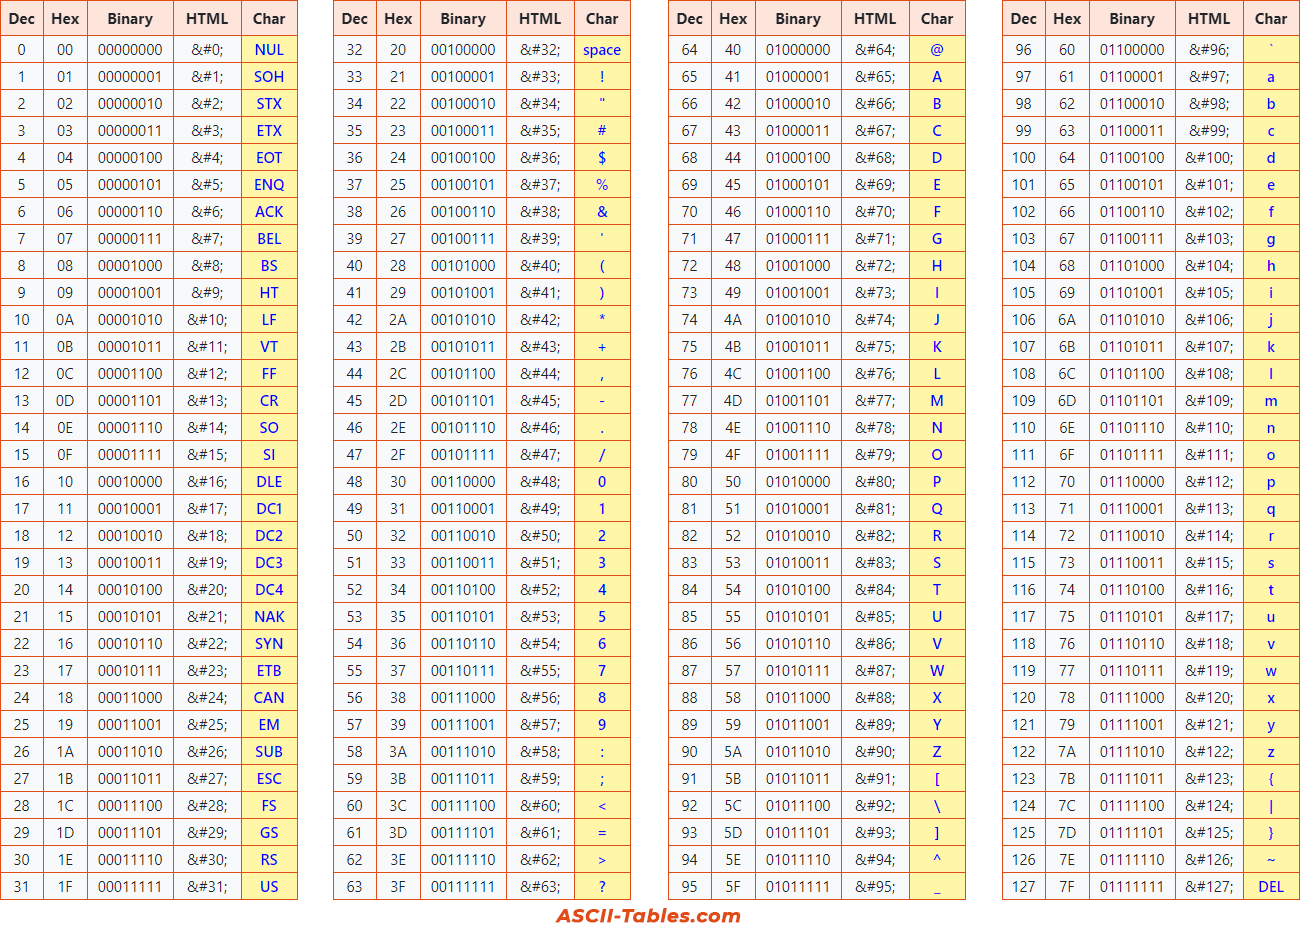
\includegraphics[scale=0.3]{../../../assets/images/table_ASCII.png}
\end{center}
Le code ASCII est suffisant pour écrire un texte en anglais ou pour
écrire un programme informatique et il est encore très largement utilisé
de nos jours, car il a l'avantage d'être léger.

Cependant, il est insuffisant pour représenter d'autres langues que
l'anglais : pas de caractères accentués, de c-cédille, pas de caractères
grecs, hébreux, arabes, chinois, \ldots{}

\hypertarget{le-code-iso-8859-1}{%
\subsection*{2. Le code ISO-8859-1}\label{le-code-iso-8859-1}}

Pour encoder les langues européennes occidentales, plusieurs extensions
du code ASCII ont été définies par l'ISO, comme notamment la norme
ISO-8859-1 (appelée aussi ISO-Latin-1). Avec cette norme :

\begin{itemize}
\tightlist
\item
  le codage des caractères présents dans la table ASCII est conservé ;
\item
  chaque caractère est toujours codé sur un octet.
\end{itemize}

On exploite le bit de poids fort inutilisé par le codage ASCII : cela
permet de coder \(2^8=256\) caractères, soir deux fois plus qu'avec le
code ASCII.

\hypertarget{le-code-unicode}{%
\subsection*{3. Le code Unicode}\label{le-code-unicode}}

Ces extensions du code ASCII ne suffisent évidemment pas à encoder les
caractères des langues non latines. Il a donc fallu créer une autre
norme internationale : la norme \textbf{Unicode}, apparue au début des
années 90.

Dans sa version 14.0 publiée en septembre 2021, la table Unicode compte
144 697 caractères couvrant plus de 150 écritures.

Unicode est une table qui regroupe tous les caractères existant au monde,
mais ne s'occupe pas de la façon dont les caractères sont codés dans la
machine. Il existe pour cela plusieurs formats différents, le plus
répandu étant l'encodage \textbf{UTF-8}.

\textbf{UTF-8} est un code à taille variable dans lequel les caractères
sont représentés sur 1, 2, 3 ou 4 octets.

Les 128 premiers caractères de la table UTF-8 sont compatibles avec le
codage ASCII. Ainsi le codage UTF-8 d'un texte ne comportant que des
caractères présents dans la table ASCII sera le même que le codage ASCII
de ce texte.

Ce ne sera pas vrai pour un texte ISO-8859-1.

\newpage

Il importe donc, quand on veut décoder un texte, de savoir quel est le
codage utilisé sous peine de décoder improprement les caractères, ce qui
arrive par exemple lorsque l'encodage d'une page web n'est pas bien
reconnu par le navigateur :

\begin{center}
  

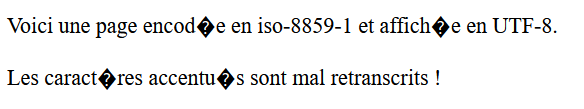
\includegraphics[scale=0.75]{../../../assets/images/erreur_encodage.png}
\end{center}

On représente en général un code UTF-8 sous la forme \texttt{U+XXXX} où
XXXX est un nombre écrit en hexadécimal.

En voici quelques exemples :

\begin{center}
  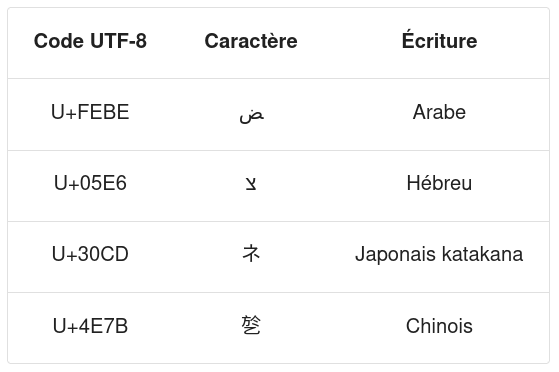
\includegraphics[scale=0.5]{tab_unicode.png}
\end{center}

Le site \url{unicode-table.com/fr} liste tous les caractères de la
table Unicode.

\medskip

\begin{remarque}{}
Remarque Depuis sa version 3, Python utilise l'encodage UTF-8 pour les
chaînes de caractères.

Nous disposons en Python de deux fonctions liées à ce codage :

\begin{itemize}
\tightlist
\item
  \texttt{chr(x)} : retourne le caractère codé par l'entier \(x\) écrit
  en base 10 ;
\item
  \texttt{ord(c)} : retourne l'entier correspondant au caractère c (de
  type str).
\end{itemize}

\begin{center}
\begin{minipage}{3cm}
\begin{minted}[frame=leftline,framerule=2pt,rulecolor=Gray!90,bgcolor=Gray!15]{pycon}
>>> chr(244)
'ô'
>>> ord("€")
8364
\end{minted}
\end{minipage}
\end{center}

\end{remarque}

\hypertarget{convertir-un-fichier-dun-encodage-uxe0-un-autre}{%
\subsection*{4. Convertir un fichier d'un encodage à un
autre}\label{convertir-un-fichier-dun-encodage-uxe0-un-autre}}

Pour convertir un fichier d'un encodage à un autre, on peut utiliser
l'éditeur Notepad++ dans lequel on trouve un menu ``Encodage''
comprenant par exemple une commande ``convertir en UTF-8''.

\begin{center}
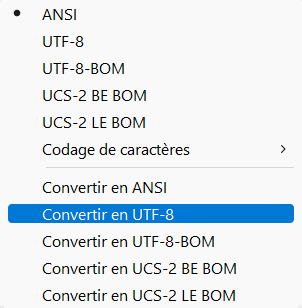
\includegraphics[scale=0.5]{../../../assets/images/notepad_encodage.png}
\end{center}

\hypertarget{ouverture-dun-fichier-texte-en-python}{%
\subsection*{5. Ouverture d'un fichier texte en
Python}\label{ouverture-dun-fichier-texte-en-python}}

Une bonne compréhension du problème de l'encodage des caractères permet
d'éviter certaines erreurs lors de l'utilisation de fichiers textes en
Python.

Considérons par exemple deux fichiers textes \texttt{texte\_ascii.txt}
et \texttt{texte\_utf-8.txt} contenant le même texte, l'un étant encodé
en ASCII étendu (c'est-à-dire en ISO-8859-1) et l'autre en UTF-8.

Le programme ci-dessous ouvre ces fichiers l'un après l'autre et affiche
leur contenu dans la console interactive.

\begin{center}
\begin{minipage}{6cm}
\begin{minted}[frame=leftline,framerule=2pt,rulecolor=Gray!90,bgcolor=Gray!15]{python}
from io import open

f = open("texte_ascii.txt")
for ligne in f.readlines():
    print(ligne)
f.close()

print("---------")

f = open("texte_utf-8.txt")
for ligne in f.readlines():
    print(ligne)
f.close()
\end{minted}
\end{minipage}
\end{center}

Tout d'abord, le programme est exécuté sous Windows :

\begin{center}
\begin{minipage}{11cm}
\begin{minted}[frame=leftline,framerule=2pt,rulecolor=Gray!90,bgcolor=Gray!15]{pycon}
Ceci est un fichier texte

encodé au format ASCII étendu

Voici quelques mots avec des caractères spéciaux

comme par exemple forçat ou encore Niño ...
---------
Ceci est un fichier texte

encodé au format UTF-8 étendu

Voici quelques mots avec des caractères spéciaux

comme par exemple forçat ou encore Niño ...
\end{minted}
\end{minipage}
\end{center}

Et maintenant sous Linux :

\begin{center}
\begin{minipage}{18cm}
\begin{minted}[frame=leftline,framerule=2pt,rulecolor=Gray!90,bgcolor=Gray!15]{python}
Traceback (most recent call last):
  File "/usr/lib/python3.10/idlelib/run.py", line 578, in runcode
    exec(code, self.locals)
  File "/home/fabrice/windows/lecture_fichier.py", line 4, in <module>
    for ligne in f.readlines():
  File "/usr/lib/python3.10/codecs.py", line 322, in decode
    (result, consumed) = self._buffer_decode(data, self.errors, final)
UnicodeDecodeError: 'utf-8' codec can't decode byte 0xe9 in position 32: invalid ...
\end{minted}
\end{minipage}
\end{center}

Pourquoi cette différence ? La fonction \texttt{open} de Python essaie
de lire le fichier texte en utilisant l'encodage du système
d'exploitation dans lequel Python est utilisé.

\begin{itemize}
\tightlist
\item
  Sous Windows, l'encodage du système est un dérivé de ISO-8859-1. Le
  fichier ASCII est donc bien lu et affiché, le fichier UTF-8, lui, est
  bien lu, mais les caractères ne sont pas affichés correctement.
\item
  Sous Linux, l'encodage du système est UTF-8. Le fichier ASCII provoque
  une erreur en lecture car Python s'attend par défaut à lire des
  caractères encodés en UTF-8.
\end{itemize}

Pour éviter ce type de problème et assurer la portabilité d'un programme
d'un système d'exploitation à un autre, il est préférable de toujours
indiquer l'encodage à la fonction \texttt{open}. Le programme suivant
fonctionnera sous les deux systèmes et provoquera l'affichage attendu.

\begin{center}
\begin{minipage}{11cm}
\begin{minted}[frame=leftline,framerule=2pt,rulecolor=Gray!90,bgcolor=Gray!15]{python}
from io import open

f = open("texte_ascii.txt", encoding="ISO-8859-1")
for ligne in f.readlines():
    print(ligne)
f.close()

print("---------")

f = open("texte_utf-8.txt", encoding="UTF-8")
for ligne in f.readlines():
    print(ligne)
f.close()
\end{minted}
\end{minipage}
\end{center}

\begin{center}
\begin{minipage}{11cm}
\begin{minted}[frame=leftline,framerule=2pt,rulecolor=Gray!90,bgcolor=Gray!15]{pycon}
Ceci est un fichier texte

encodé au format ASCII étendu

Voici quelques mots avec des caractères spéciaux

comme par exemple forçat ou encore Niño ...
---------
Ceci est un fichier texte

encodé au format UTF-8 étendu

Voici quelques mots avec des caractères spéciaux

comme par exemple forçat ou encore Niño ...
\end{minted}
\end{minipage}
\end{center}

\end{document}